\documentclass[12pt]{article}
\usepackage[paper=letterpaper,margin=2cm]{geometry}
\usepackage{amsmath}
\usepackage{amssymb}
\usepackage{amsfonts}
\usepackage{newtxtext, newtxmath}
\usepackage{enumitem}
\usepackage{titling}
\usepackage[colorlinks=true]{hyperref}
\usepackage[T1]{fontenc}
\usepackage{listings}
\usepackage{color}
\usepackage{graphicx}
\usepackage{tikz}
\usepackage{multicol}

\definecolor{dkgreen}{rgb}{0,0.6,0}
\definecolor{gray}{rgb}{0.5,0.5,0.5}
\definecolor{mauve}{rgb}{0.58,0,0.82}

\lstset{frame=tb,
  language=Python,
  upquote=true,
  showstringspaces=false,
  columns=flexible,
  basicstyle={\small\ttfamily},
  numbers=left,
  numberstyle=\tiny\color{gray},
  keywordstyle=\color{blue},
  commentstyle=\color{dkgreen},
  stringstyle=\color{mauve},
  breaklines=true,
  breakatwhitespace=true,
  tabsize=2,
  backgroundcolor=\color{white},   % choose the background color
  captionpos=b,                    % sets the caption-position to bottom
  escapeinside={\%*}{*)},          % if you want to add LaTeX within your code
}

\begin{titlepage}
  \title{Introduction to AI}
  \author{Assignment 2}
  \date{\today}
\end{titlepage}

\begin{document}
\maketitle
\begin{enumerate}
  % \usetikzlibrary{positioning, quotes}
\item For\footnote{Source code on \url{https://github.com/jinhanloh2021/AI\_AS2}} the below graph (heuristic values are provided in red color and actual costs are in black
color), please provide answers to the following answers:\\
Please note that $S$ is start and $G$ is the goal state.
\begin{center}
  \begin{tikzpicture}[
      ->,>=stealth,auto,node distance=0cm,
      thick,main node/.style={circle,draw}
    ]
    \node[main node][label={[font=\small,text=red]above:$14$}] (S) at (0,3){$S$};
    \node[main node][label={[font=\small,text=red]below:$8$}] (A) at (3,0){$A$};
    \node[main node][label={[font=\small,text=red]above right:$10$}] (B) at (3,3){$B$};
    \node[main node][label={[font=\small,text=red]above:$10$}] (C) at (3,6){$C$};
    \node[main node][label={[font=\small,text=red]below:$6$}] (D) at (6,0){$D$};
    \node[main node][label={[font=\small,text=red]above right:$4$}] (E) at (6,3){$E$};
    \node[main node][label={[font=\small,text=red]above:$6$}] (F) at (6,6){$F$};
    \node[main node][label={[font=\small,text=red]above:$1$}] (H) at (9,3)  {$H$};
    \node[main node] (G) at (12,3){$G$};

    \draw [->]
    (S)  edge["6"] (A)
    (S)  edge["4"] (B)
    (S)  edge["9"] (C)
    (A)  edge["2"] (D)
    (B)  edge["6"] (E)
    (C)  edge["4"] (F)
    (B)  edge["1"] (A)
    (B)  edge["1"] (C)
    (A)  edge["4"] (E)
    (C)  edge["4"] (E)
    (F)  edge["1"] (E)
    (D)  edge["1"] (E)
    (D)  edge["5"] (H)
    (E)  edge["3"] (H)
    (F)  edge["5"] (H)
    (H)  edge["3"] (G);
  \end{tikzpicture}
\end{center}
\begin{enumerate}
  \item Is the heuristic admissible? Provide justification. Please fill in the intermediate table below to answer this question.
        \begin{center}
          \bgroup
          \def\arraystretch{1.5}%
          \captionsetup{type=figure}
          \begin{tabular}{|c|c|c|}
            \hline
            Node $n$ & Min cost to reach $G$ from $n$ & $h(n)$ \\
            \hline
            $S$      & $14$                           & $14$   \\
            $A$      & $9$                            & $8$    \\
            $B$      & $10$                           & $10$   \\
            $C$      & $10$                           & $10$   \\
            $D$      & $7$                            & $6$    \\
            $E$      & $6$                            & $4$    \\
            $F$      & $7$                            & $6$    \\
            $H$      & $3$                            & $1$    \\
            \hline
          \end{tabular}
          \captionof{table}{Comparison of min cost to goal and heuristic for every node}
          \egroup
        \end{center}
        Since $\forall n$, $h(n)\le Mincost(n)$, the heuristic $h$ is admissible.
  \item Is the heuristic consistent? Provide justification.\\[10pt]
        A heuristic is consistent if $\forall n \ \text{and}\  \forall p$, $h(n) \le c(n,p) + h(p)$. For the given graph, the heuristic $h$ is not consistent. This can be proven by counter-example.\\
        Take node $B$ and $A$. Given
        \begin{align*}
          h(B)   & = 10 \\
          c(B,A) & = 1  \\
          h(A)   & = 8  \\
        \end{align*}
        Then
        \begin{align*}
          h(B) & > c(B,A) + h(A) \\
          10   & > 8 + 1 = 9     \\
        \end{align*}
        Hence, $h$ is not consistent.
  \item Provide the search steps (as discussed in class) with vanilla \textbf{Breadth First Search (BFS)}. Show the \textbf{final solution path} and the \textbf{cost of that solution} for each algorithm. Also compute the search steps for \textbf{A* search} with the following heuristic:\\[10pt]
        Specify for each algorithm if the open list is queue, stack or priority queue. As a simplifying assumption, let index zero (i.e first element) in the open list be the top of the stack or front of the (priority) queue, as appropriate for the corresponding algorithm. Break ties by alphabetical order.\\
        Please use the following tables for your working. Open list contains nodes that are to be explored, and "nodes to add" are the successors of the node that is recently popped or dequeued.\\[10pt]
        \textbf{Breadth First Search algorithm}
        \begin{center}
          \bgroup
          \def\arraystretch{1.5}%
          \captionsetup{type=figure}
          \begin{tabular}{|c|c|c|c|}
            \hline
            Step \# & Open Queue           & Dequeue & Nodes to add \\
            \hline
            $1$     & $S$                  & $S$     & $A,B,C$      \\
            $2$     & $A^S, B^S, C^S$      & $A$     & $D,E$        \\
            $3$     & $B^S, C^S, D^A, E^A$ & $B$     &              \\
            $4$     & $C^S, D^A, E^A$      & $C$     & $F$          \\
            $5$     & $D^A, E^A, F^C$      & $D$     & $H$          \\
            $6$     & $E^A, F^C, H^D$      & $E$     &              \\
            $7$     & $F^C, H^D$           & $F$     &              \\
            $8$     & $H^D$                & $H$     & $G$          \\
            $9$     & $G^H$                & $G$     &              \\
            \hline
          \end{tabular}
          \captionof{table}{BFS priority queue}
          \egroup
        \end{center}
        Path taken is
        $$
          S \rightarrow A \rightarrow D \rightarrow H \rightarrow G
        $$
        \begin{align*}
          cost & = 6 + 2 + 5 + 3 \\
               & = 16
        \end{align*}
        \textbf{A* Search algorithm}\\
        Let $X^n_f$ be a node $X$, where $n$ is the parent state and $f=g(X) + h(X)$ as defined by the algorithm.
        \begin{center}
          \bgroup
          \def\arraystretch{1.5}%
          \captionsetup{type=figure}
          \begin{tabular}{|c|c|c|c|}
            \hline
            Step \# & Open Priority Queue                      & Dequeue & Nodes to add \\
            \hline
            $1$     & $S$                                      & $S$     & $A,B,C$      \\
            $2$     & $A^S_{14}, B^S_{14}, C^S_{19}$           & $A$     & $D,E$        \\
            $3$     & $B^S_{14}, D^A_{14}, E^A_{14}, C^S_{19}$ & $B$     & $A,C$        \\
            $4$     & $A^B_{13}, D^A_{14}, E^A_{14}, C^B_{15}$ & $A$     & $D,E$        \\
            $5$     & $D^A_{13}, E^A_{13}, C^B_{15}$           & $D$     & $E,H$        \\
            $6$     & $E^D_{12}, H^D_{13}, C^B_{15}$           & $E$     & $H$          \\
            $7$     & $H^E_{12}, C^B_{15}$                     & $H$     & $G$          \\
            $8$     & $G^H_{14}, C^B_{15}$                     & $G$     &              \\
            \hline
          \end{tabular}
          \captionof{table}{A* search priority queue}
          \egroup
        \end{center}
        Path taken is
        $$
          S \rightarrow B \rightarrow A \rightarrow D \rightarrow E \rightarrow H \rightarrow G
        $$
        \begin{align*}
          cost & = 4 + 1 + 2 + 1 + 3 + 3 \\
               & = 14
        \end{align*}
\end{enumerate}
  \item You are hired by a moving company to move $N$ boxes from a corner of a room to the opposite
corner of the room. The room can be roughly divided into four corners, and there is an indoor
pond in the middle of the room preventing any direct diagonal crossing. The three boxes have
different sizes and can only be stacked in such a way that larger boxes can never be placed
on top of smaller ones.\\
Please answer the following questions:
\begin{enumerate}
  \item Given $N$ boxes (stacked appropriately in corner $A$ with the smallest box on the top), formulate this problem as a search problem. Indicate the
        \begin{itemize}
          \item States (describe specifically what a state is in this problem, how you would store it in a computer using a data structure, and justify the correctness of your representation)
          \item Actions
          \item Cost of different actions
          \item Successor state for each action and give one example with all of its successor states listed
          \item The objective
        \end{itemize}
        I made some assumptions for this problem:
        \begin{itemize}
          \item I can only move one box at a time
          \item I can only remove a box from the top of a stack
          \item I can only add a box to the top of a stack
          \item I cannot sort a stack in place
          \item Each room can only contain one stack
          \item All boxes have unique sizes
          \item All stacks must be appropriately placed, smallest box at top largest at bottom
        \end{itemize}
        With the rules of the game clear, we can define the state unambiguously.\\
        Let the set of rooms be $R = \{a, b, c, d\}$, a box $B$ with size $i$ be $b_i\in B=\{b_1, b_2, \ldots ,b_n\}$, a stack $G$ in room $r$ be $g(r) \subseteq B$ and a box $b_i$ in a stack $g(r)$ be $g(r,i)\in B$, the number of boxes be $N$, and the position of the mover $M$ in the room $r$ be $M = m_r$.\\
        We can then represent the start state as with $N=3$ as
        \begin{align*}
          g(a) & = \{b_1, b_2, b_3\} \\
          g(b) & = \{\emptyset\}     \\
          g(c) & = \{\emptyset\}     \\
          g(d) & = \{\emptyset\}     \\
          M    & = m_a
        \end{align*}
        And the goal state as the state where all boxes are in $g(d)$
        \begin{align*}
          g(a) & = \{\emptyset\}     \\
          g(b) & = \{\emptyset\}     \\
          g(c) & = \{\emptyset\}     \\
          g(d) & = \{b_1, b_2, b_3\} \\
          M    & = m_d
        \end{align*}
        This represents 4 stacks $g(r)$ in each room $R = \{a, b, c, d\}$, with a set of boxes. Each stack must be ordered from smallest to largest. And $M$ represents the position of the mover.\\
        To represent the state as a data structure in Python, we can use a list containing 4 stacks. Each stack represents the stack of boxes in a room. We can assign each room to each stack respectively in increasing order. The stack is implemented as an integer list and each integer represents the size of a box. The mover can be represented as a separate integer variable containing the index of the stack he is in. Here is a diagram to illustrate this model.
        \begin{center}
          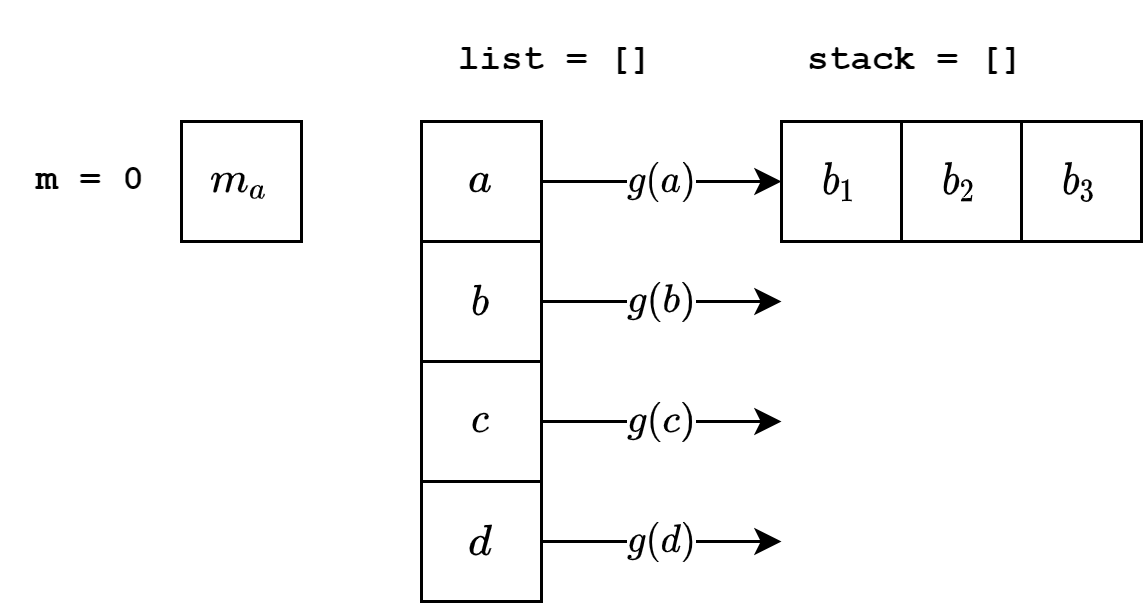
\includegraphics[scale=0.3]{"./Diagrams/Q2_DataStructure.png"}
        \end{center}
        This data structure is correct because it contains all possible positions of the boxes in every room. It also contains all possible rooms the mover can be in. It does not enforce the constraints such as the ordering or the diagonal constraint. These will be enforced by the methods we are allowed to perform on the data structure.\\
        The base action in our system is to move a box from one room to an adjacent room, subject to the system rules. This action has a cost 1. We further simplify the actions by assuming that:
        \begin{itemize}
          \item The size of the box doesn't affect the cost
          \item Moving without a box has 0 cost
          \item Appending and popping from a stack (picking up and putting down a box) costs 0
          \item Mover must be in the same room as a box to pick up or put down a box
        \end{itemize}
        For example, for an action $C(a, b), C(b, d)$ represents popping a box from the top of the stack $g(a)$ and carrying it to room $b$, then carrying it to room $d$ and appending it to the top of the stack $g(d)$. The popping and appending costs 0. The moving has a cost of $1+1=2$ as we travelled from $a\rightarrow b$ and from $b\rightarrow d$. In the implementation, there must be checks to ensure that the ordering rule is respected when appending to a stack.\\
        Here is an example of a state with $N=1$ and all successor states.
        \begin{center}
          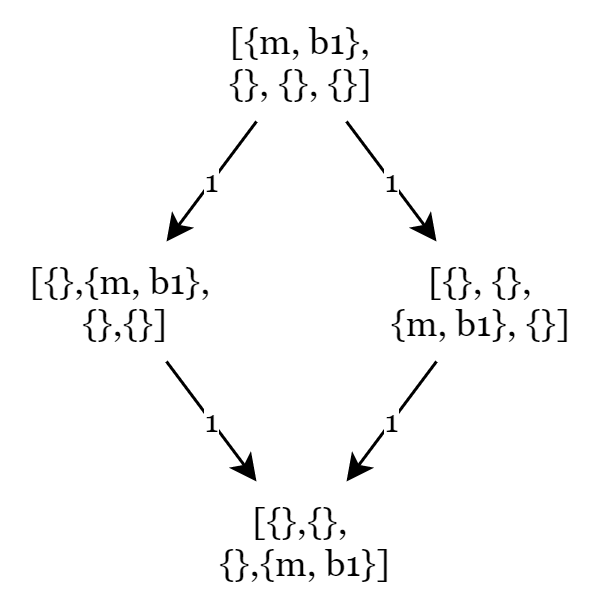
\includegraphics[scale=0.4]{"./Diagrams/Q2_StartStateWithAllSuccessorStates.png"}
        \end{center}
        This represents a start state where one box $b_1$ is in room $a$ and the mover is also in room $a$. The possible actions from the start state are to move the box to rooms $b$ or $c$, then to $d$.\\
        We can see that we have reached the goal state by completing action in two steps as all the boxes are in the room $d$.
  \item For using heuristic search methods such as A*, provide an admissible heuristic and justify why it is admissible.\\[10pt]
        An admissible heuristic for some state $n$ would be the number of boxes not in room $d$.
        $$
          h(n) = N - \lvert g(d)\rvert
        $$
        Given a base case where we have a single box in room $b$, the least cost path is 1, which is to take the box directly to $C(b,d)$. But for any other case where we have more than 1 box or if our box is located diagonally from the $d$, the cost would be greater as we cannot directly append the boxes to stack $g(d)$ as it will violate the ordering rule. We might also have to travel more than one room to reach $d$.\\
        This will always result in a cost greater than the heuristic.Thus the heuristic admissible.
  \item For the case where $N = 3$, compute the first three steps of DFS search. You can use the table structure as in question 1c to show different steps.
        \begin{center}
          \bgroup
          \def\arraystretch{1.5}%
          \captionsetup{type=figure}
          \begin{tabular}{|c|c|}
            \hline
            Step \# & Stacks                                    \\
            \hline
            $1$     & $[\{m,b_1, b_2, b_3\}, \{\}, \{\}, \{\}]$ \\
            $2$     & $[\{b_2, b_3\}, \{m,b_1\}, \{\}, \{\}]$   \\
            $3$     & $[\{m,b_2, b_3\}, \{b_1\}, \{\}, \{\}]$   \\
            \hline
          \end{tabular}
          \captionof{table}{States of stacks for first three steps of DFS}
          \egroup
        \end{center}
  \item Give a solution to the problem for $N = 3$. You can achieve it either using some methods from the class or through guessing.
        I am ignoring the position of the mover $m$ in the state here as his movement without a box costs 0. To transition from a state $[\{b_2, b_3\}, \{m,b_1\}, \{\}, \{\}]$ to $[\{m,b_2, b_3\}, \{b_1\}, \{\}, \{\}]$ costs 0, so I will omit it for brevity's sake.
        \begin{center}
          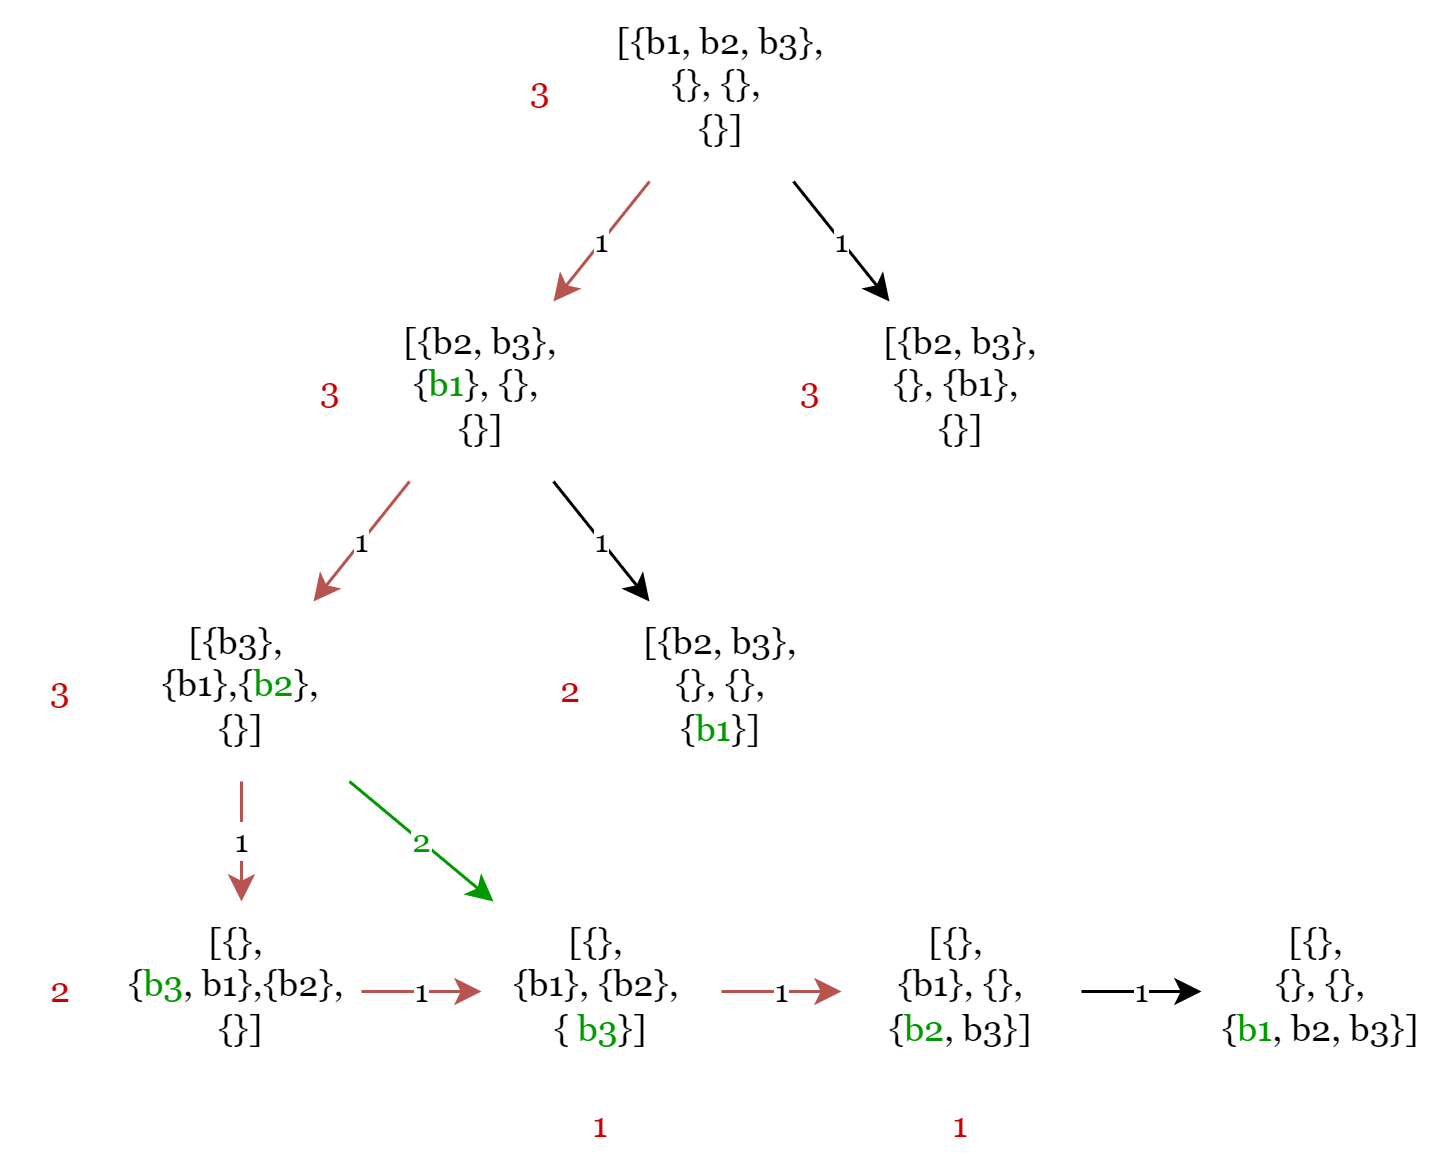
\includegraphics[scale=0.25]{"./Diagrams/DFS_Tree_Solution.png"}
        \end{center}
        The solution is shown by the red arrows. The cost of each action is shown in the arrow as black text, and the red text represents the heuristic of each state. The green elements highlights the box that is currently held by the mover. There is a green arrow which represents a "shortcut" as the mover moves from $a$ to $d$ through $c$. Note that in $[\{\}, \{b_3, b_1\}, \{b_2\}, \{\}]$ the order rule appears to be violated as $b_3$ is above $b_1$. But since the box $b_3$ is being held by the mover in room $b$, it is not violated.
  \item How would the state representation change in part A if the following modifications are applied to the problem:
        \begin{itemize}
          \item The cost to move one box is now proportional to the size of the box (cost of 1 for moving the smallest box, cost of 3 for moving the largest one).
          \item If the moving company employee moves from one corner to the other without carrying any box, it also incurs a cost of 0.5
        \end{itemize}
        For my state representation, the box representation will still work as my boxes are labelled as $b_i$ where $i$ is the weight. Similarly, the position of the mover is still the same with the new rule that movement from one corner to another without a box will cost 0.5.\\[10pt]
        The changes can be seen in the \textbf{actions} rather than in the state. Now we can redefine an action to $C(a,b,b_i)$, where the mover moves a box $b_i$ from room $a$ to $b$. Previously the cost was $1$ for any $b_i$ but the new cost will be $i$.\\
        Another change we have to make is to represent the position of the mover. Previously I ignored his position in our state representation as his movement cost without a box was 0. But now, we can have a new action $C(a,b,b_0)$ which costs 0.5, when a mover moves from room $a$ to room $b$ without a box. Now we cannot ignore the position of the mover, and we require an additional variable in our state $m$ to represent the room the mover is currently in.
\end{enumerate}
  % \item\footnote{Full submission can be found on \url{https://github.com/jinhanloh2021/AI\_AS1}} Write True/False for the following conditional independence statements. Justify clearly your answer by showing active/blocked trails as necessary and appropriate rules for them to be active/blocked. [No coding required for this question. Each sub-question has \textbf{2 points}]

\begin{enumerate}
      \item $A \perp G \mid \{F\}$\\
            False. There is a V-structure between $A$ and $G$.
            $$A \rightarrow B \rightarrow D \leftarrow G$$
            Given $F$ and thus implying we know $D$, it couples $A$ and $G$. Thus $A$ and $G$ are dependent.
      \item $A \perp G \mid \{E\}$\\
            False. There is a common cause structure.
            $$A \leftarrow C \rightarrow E \rightarrow G$$
            $A$ and $E$ are dependent, and thus by cascade structure $A$ and $G$ are also dependent. But given $E$, it blocks the active path between $A$ and $G$. Thus $A$ and $G$ are independent given $E$.
      \item $A \perp E \mid \{C\}$\\
            True. $A$, $C$ and $E$ have a common cause structure.
            $$A \leftarrow C \rightarrow E$$
            Given the common cause $C$, it decouples $A$ and $E$. There are no other active paths between $A$ and $C$, thus they are independent.
      \item $A \perp E \mid \{C, D\}$\\
            False. Similar to part (c), given $C$ it decouples $A$ and $E$ at $A \leftarrow C \rightarrow E$. However, there exists a V-structure between $A$ and $E$.
            $$A \rightarrow B \rightarrow D \leftarrow E$$
            Similar to part (a), given $D$ it couples $A$ and $E$. Thus $A$ and $E$ are dependent.
      \item $A \perp D \mid \{B, E\}$\\
            True. Cascade from $A \rightarrow B \rightarrow D$ is blocked given $B$. Common cause couples $A$ and $E$. But path from $A \leftarrow C \rightarrow E \rightarrow D$ is blocked given $E$. Since all paths from $A$ to $D$ are blocked, $A$ and $D$ are independent.
\end{enumerate}
\clearpage
  % \item
\begin{enumerate}
  \item Draw the Bayes net corresponding to this setup. {\bf [3 points]}
        \begin{center}
          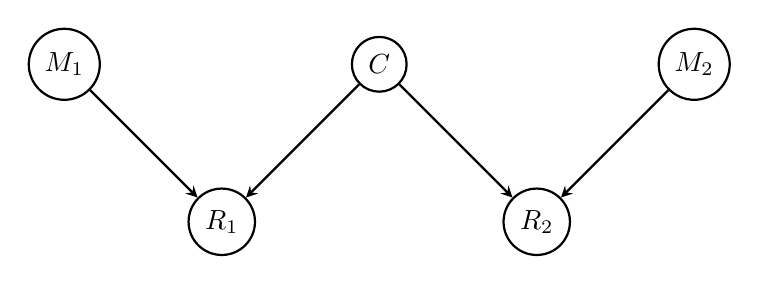
\begin{tikzpicture}[->,>=stealth,auto,node distance=0cm,
              thick,main node/.style={circle,draw}]

            \node[main node] (M1) at (0,2) {$M_1$};
            \node[main node] (R1) at (2,0) {$R_1$};
            \node[main node] (C) at (4,2) {$C$};
            \node[main node] (R2) at (6,0) {$R_2$};
            \node[main node] (M2) at (8,2) {$M_2$};

            \path[every node/.style={}]
            (M1) edge (R1)
            (C) edge (R1)
            (C) edge (R2)
            (M2) edge (R2);

          \end{tikzpicture}
        \end{center}
        \begin{center}
          \bgroup
          \def\arraystretch{1.5}%
          \begin{tabular}{|c|c|p{6cm}|}
            \hline
            Variable Name & Domain        & Interpretation                                                               \\
            \hline
            $C$           & $\{1, 0\}$    & The actual health of a person. Either COVID positive $1$ or negative $0$.    \\
            \hline
            $M_1$         & $\{a, b, c\}$ & The manufacturer of the first test kit. Where the company is $a, b$ or $c$.  \\
            \hline
            $M_2$         & $\{a, b, c\}$ & The manufacturer of the second test kit. Where the company is $a, b$ or $c$. \\
            \hline
            $R_1$         & $\{1, 0\}$    & The result of the first test kit. Either positive $1$ or negative $0$.       \\
            \hline
            $R_2$         & $\{1, 0\}$    & The result of the second test kit. Either positive $1$ or negative $0$.      \\
            \hline
          \end{tabular}
          \egroup
        \end{center}
        This table can be interpreted as three independent events $M_1$, $M_2$ and $C$. The manufacturer of the two test kits received by a person and their actual health are independent, but they will determine the result of the test kit.
  \item Write conditional probabilities (numerical values) associated with each node of this Bayes net. As there are 5 variables, please specify one conditional probability table (CPT) for each variable. {\bf [2 points]}
        \begin{center}
          \bgroup
          \def\arraystretch{1.5}%
          \begin{tabular}{|c|c|c|}
            \hline
            $P(C=0)$ & $P(C=1)$ \\
            \hline
            $0.7$    & $0.3$    \\
            \hline
          \end{tabular}
          \egroup
        \end{center}
        \begin{center}
          \begin{center}
            \bgroup
            \def\arraystretch{1.5}%
            \begin{tabular}{|c|c|c|}
              \hline
              $P(M_n=a)$ & $P(M_n=b)$ & $P(M_n=c)$ \\
              \hline
              $0.333$    & $0.333$    & $0.333$    \\
              \hline
            \end{tabular}
            \egroup
          \end{center}
          \bgroup
          \def\arraystretch{1.5}%
          \begin{tabular}{|cc|c|c|}
            \hline
            $M_n$ & $C$ & $P(R_n=0\mid M_n, C)$ & $P(R_n=1\mid M_n, C)$ \\
            \hline
            $a$   & $0$ & $0.99$                & $0.01$                \\
            \hline
            $b$   & $0$ & $0.95$                & $0.05$                \\
            \hline
            $c$   & $0$ & $0.91$                & $0.09$                \\
            \hline
            $a$   & $1$ & $0.3$                 & $0.7$                 \\
            \hline
            $b$   & $1$ & $0.2$                 & $0.8$                 \\
            \hline
            $c$   & $1$ & $0.1$                 & $0.9$                 \\
            \hline
          \end{tabular}
          \egroup
        \end{center}
        For values of $n \in \{1, 2\}$ as each person has two test kits.
  \item Are the results of the two tests dependent or independent given the evidence that the Covid Status is known? Justify your answer. {\bf [1 point]}\\[5pt]
        There is a common cause structure $R_1 \leftarrow C \rightarrow R_2$ which couples $R_1$ and $R_2$. But given the COVID status $C$, it decouples $R_1$ and $R_2$. Thus they are independent.
  \item Assume you took both tests at home. After being tested twice in a matter of minutes, the first test was positive and the second negative. What is the probability that you actually have COVID19? Show your analytical computations. {\bf [4 points]}\\[5pt]
        Given that the first test was positive and the second test was negative, then
        \begin{align*}
          R_1 & =1 \\
          R_2 & =0
        \end{align*}
        We are trying to solve for $P(C=1\mid R_1=1, R_2=0)$. Since $R_1$ and $R_2$ are conditionally independent on $C$,
        \begin{align*}
          P(C=1\mid R_1=1, R_2=0) & =\frac{P(R_1=1, R_2=0\mid C=1)P(C=1)}{P(R_1=1, R_2=0)}          \\[5pt]
                                  & =\frac{P(R_1=1\mid C=1)P(R_2=0\mid C=1)P(C=1)}{P(R_1=1, R_2=0)}
        \end{align*}
        To find $P(R_1=1\mid C=1)$ and $P(R_2=0\mid C=1)$, marginalise over the manufacturer $M$.
        \begin{align*}
          P(R_1=1\mid C=1) & =\frac{0.7+0.8+0.9}{(0.1+0.2+0.3)+(0.7+0.8+0.9)} \\[5pt]
                           & =0.8                                             \\
          P(R_2=0\mid C=1) & = 1-0.8                                          \\
                           & =0.2
        \end{align*}
        Thus we have solved for numerator,
        \begin{align*}
          P(R_1=1\mid C=1)P(R_2=0\mid C=1)P(C=1) & = (0.8)(0.2)(0.3) \\
                                                 & =0.048
        \end{align*}
        To solve for the denominator, it is the {\it hard part}. We cannot use marginalisation as there are too many varibales to sum over. We can use variable elimination instead. The joint distribution is
        \begin{align*}
            & P(C=c, M_1=m_1, M_2=m_2, R_1=r_1, R_2=r_2)                              \\
          = & P(C=c)P(M_1=m_1) P(M_2=m_2) P(R_1=r_1\mid C, M_1) P(R_2=r_2\mid C, M_2)
        \end{align*}
        Then,
        \begin{align*}
            & P(R_1=1, R_2=0)                                                                                                           \\[5pt]
          = & \sum_{C, M_1, M_2}P(C=c)P(M_1=m_1) P(M_2=m_2) P(R_1=1\mid C, M_1) P(R_2=0\mid C, M_2)                                     \\[5pt]
          = & \sum_{C, M_1}P(C=c)P(M_1=m_1)P(R_1=1\mid C,M_1)\underbrace{\sum_{M_2}P(M_2=m_2)P(R_2=0\mid C, M_2)}_{\tau_1(R_2=0\mid C)} \\[5pt]
          = & \sum_{C}P(C=c)\tau_1(R_2=0\mid C)\underbrace{\sum_{M_1}(M_1=m_1)P(R_1=1\mid C,M_1)}_{\tau_2(R_1=1\mid C)}                 \\[5pt]
          = & \sum_{C}P(C=c)\tau_1(R_2=0\mid C)\tau_2(R_1=1\mid C)                                                                      \\[5pt]
        \end{align*}
        Calculate the case where $C=0$,
        \begin{align*}
          P(R_1=1 \mid C=0) & = \frac{0.01+0.05+0.09}{(0.01+0.05+0.09)+(0.99+0.95+0.91)} \\
                            & = 0.05                                                     \\
          P(R_1=0 \mid C=0) & = 1 - 0.05                                                 \\
                            & =0.95                                                      \\
        \end{align*}
        Then using both cases,
        \begin{align*}
          P(R_1=1, R_2=0) & = \sum_{C}P(C=c)\tau_1(R_2=0\mid C)\tau_2(R_1=1\mid C) \\[5pt]
                          & =(0.7)(0.95)(0.05) + (0.3)(0.8)(0.2)                   \\
                          & =0.08125                                               \\
        \end{align*}
        Hence,
        \begin{align*}
          P(C=1\mid R_1=1, R_2=0) & =\frac{P(R_1=1\mid C=1)P(R_2=0\mid C=1)P(C=1)}{P(R_1=1, R_2=0)} \\[5pt]
                                  & =\frac{0.048}{0.08125}                                          \\[5pt]
                                  & = \frac{192}{325}                                               \\[5pt]
                                  & \approx 0.59                                                    \\
        \end{align*}
\end{enumerate}

\clearpage
  % \item
\begin{enumerate}
  \item Implement the above Bayes net with the specified conditional probabilities into pgmpy. {\bf [2.5 points]}
        \begin{center}
          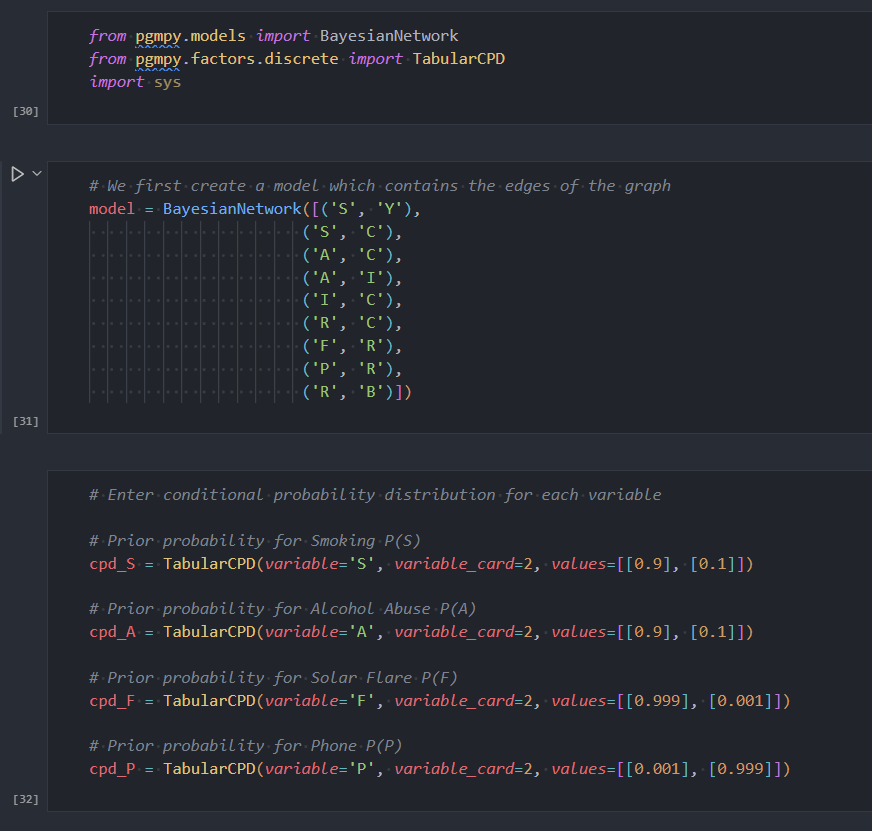
\includegraphics[scale=0.5]{"./Diagrams/Q3 Code Page 1.PNG"}
          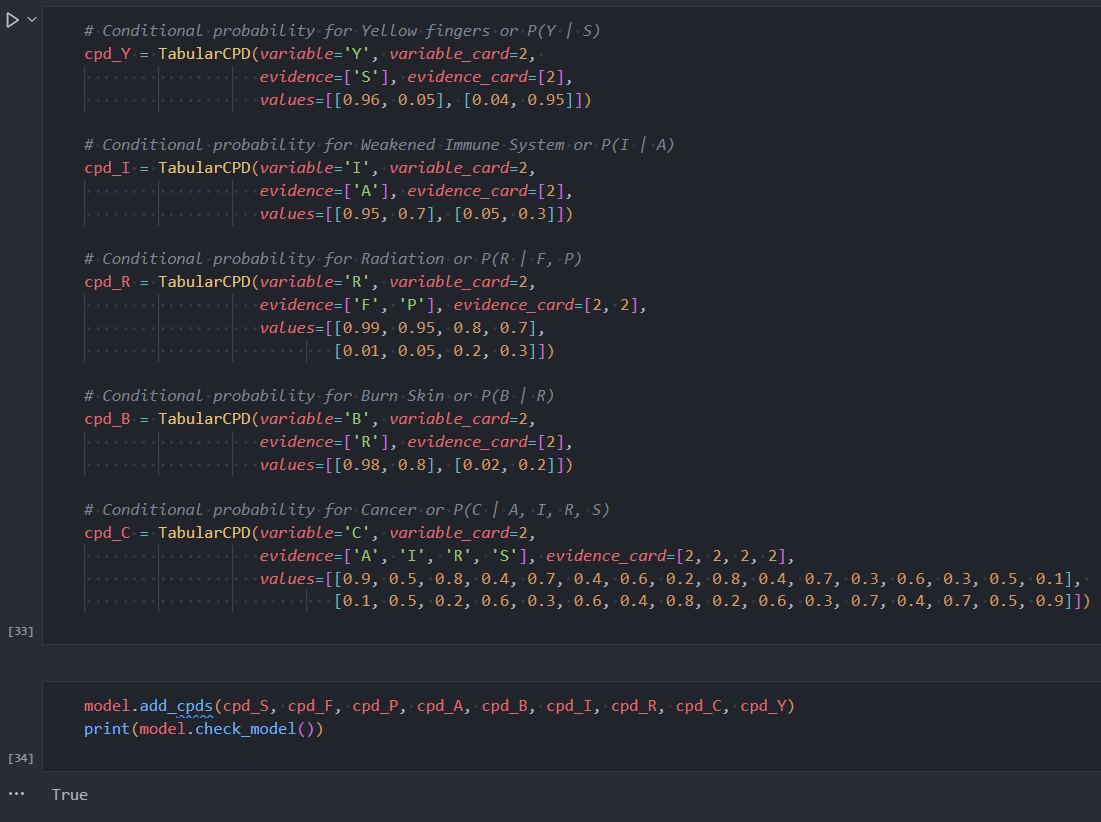
\includegraphics[scale=0.5]{"./Diagrams/Q3 Code Page 2.PNG"}
        \end{center}
        \clearpage
  \item Draw the Bayesian network clearly showing the nodes and arrows showing relationship among all the variables. {\bf [1.5 points]}
        \begin{center}
          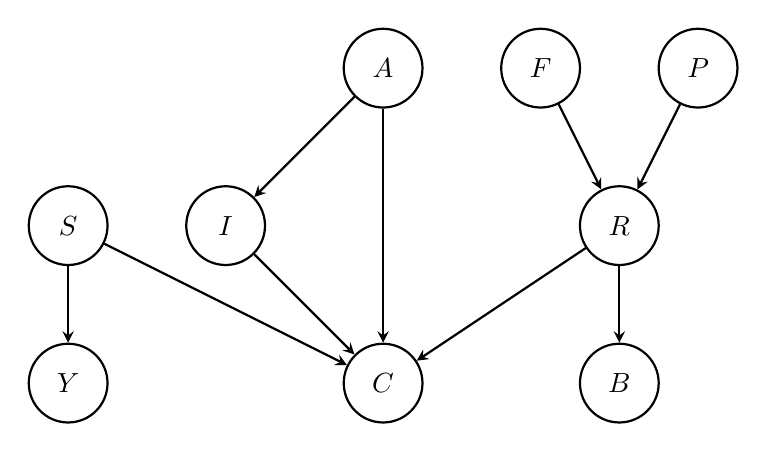
\begin{tikzpicture}[->,>=stealth,auto,node distance=0cm,
              thick,main node/.style={circle,draw}, minimum size=1cm]

            \node[main node] (S) at (0,2) {$S$};
            \node[main node] (Y) at (0,0) {$Y$};
            \node[main node] (I) at (2,2) {$I$};
            \node[main node] (A) at (4,4) {$A$};
            \node[main node] (C) at (4,0) {$C$};
            \node[main node] (F) at (6,4) {$F$};
            \node[main node] (R) at (7,2) {$R$};
            \node[main node] (B) at (7,0) {$B$};
            \node[main node] (P) at (8,4) {$P$};

            \path[every node/.style={}]
            (S) edge (Y)
            (S) edge (C)
            (A) edge (I)
            (A) edge (C)
            (I) edge (C)
            (F) edge (R)
            (P) edge (R)
            (R) edge (C)
            (R) edge (B);
          \end{tikzpicture}
        \end{center}
  \item What is the probability of radiation given cancer? Show values for $R\in\{0, 1\}$. {\bf [1.5 points]}
        $$P(R=1\mid C=1)$$
        \begin{lstlisting}
          from pgmpy.inference import VariableElimination
          infer = VariableElimination(model)

          # Get probability of Radiation given Cancer P(R=1 | C=1)
          phi_query = infer.query(['R'], evidence={'C':1}, joint = False)
          factor = phi_query['R']
          print('Probability of Radiation given Cancer')
          print(factor)

          # Output
          '''
          Probability of Radiation given Cancer
          +------+----------+
          | R    |   phi(R) |
          +======+==========+
          | R(0) |   0.9214 |
          +------+----------+
          | R(1) |   0.0786 |
          +------+----------+
          '''
        \end{lstlisting}
        \begin{align*}
          P(R=0\mid C=1) & =0.9214 \\
          P(R=1\mid C=1) & =0.0786
        \end{align*}
  \item What is the probability of cancer given the patient has skin burn, yellow fingers and abuses alcohol? Show values for $C\in\{0, 1\}$. {\bf [1.5 points]}
        $$P(C=1\mid B=1, Y=1, A=1)$$
        \begin{lstlisting}
          # Get probability of Cancer given skin burn, yellow fingers and alcohol abuse. P(C=1 | B=1, Y=1, A=1)
          phi_query = infer.query(['C'], evidence={'B':1, 'Y':1, 'A':1}, joint = False)
          factor = phi_query['C']
          print('Probability of Cancer given skin burn, yellow fingers and alcohol abuse')
          print(factor)

          # Output
          '''
          Probability of Cancer given skin burn, yellow fingers and alcohol abuse
          +------+----------+
          | C    |   phi(C) |
          +======+==========+
          | C(0) |   0.4296 |
          +------+----------+
          | C(1) |   0.5704 |
          +------+----------+
          '''
        \end{lstlisting}
        \begin{align*}
          P(C=0\mid B=1, Y=1, A=1) & =0.4296 \\
          P(C=1\mid B=1, Y=1, A=1) & =0.5704
        \end{align*}
  \item Are Smoking and skin burn independent given that cancer is present? Justify your answer. {\bf [1.5 points]}\\
        No. They are dependent.There is a V-structure between $S$, $C$ and $R$.
        $$S\rightarrow C\leftarrow R$$
        Given $C$, it couples $S$ and $R$. This makes $S$ and $R$ dependent. Since $R$ and $B$ are dependent due to cascade structure
        $$R \rightarrow B$$
        then $S$ and $B$ are dependent.
  \item What is the probability of cancer if you never abused alcohol or used a cellphone? {\bf [1.5 points]}
        $$P(C=1\mid A=0, P=0)$$
        \begin{lstlisting}
          # Get probability of Cancer given no alcohol and no cellphone. P(C=1 | A=0, P=0)
          phi_query = infer.query(['C'], evidence={'A':0, 'P':0}, joint = False)
          factor = phi_query['C']
          print('Probability of Cancer given no alcohol and no cellphone')
          print(factor)

          # Output
          '''
          Probability of Cancer given no alcohol and no cellphone
          +------+----------+
          | C    |   phi(C) |
          +======+==========+
          | C(0) |   0.8495 |
          +------+----------+
          | C(1) |   0.1505 |
          +------+----------+
          '''
        \end{lstlisting}
        \begin{align*}
          P(C=0\mid A=0, P=0) & =0.8495 \\
          P(C=1\mid A=0, P=0) & =0.1505
        \end{align*}
\end{enumerate}
  % \item You can build your solution on top of the python notebook covered in class to classify the
standard MNIST dataset.\\[5pt]
Full solution found in \lstinline{Q4_template_MNISTCorrupted.ipynb}.
\begin{lstlisting}
  from matplotlib import pyplot as plt
  import numpy as np
  import tensorflow as tf
  from tensorflow.keras import layers
  import tensorflow_datasets as tfds

  ## write your code here
  dataset_name = "mnist_corrupted/zigzag"
  train_ds = tfds.load(dataset_name, split='train', batch_size=-1, as_supervised=True)
  test_ds = tfds.load(dataset_name, split='test', batch_size=-1, as_supervised=True)

  train_images, train_labels = tfds.as_numpy(train_ds)
  test_images, test_labels   = tfds.as_numpy(test_ds)

  # Test size of different loaded numpy arrays
  print('Image size:', train_images[0].shape)
  print('Training data size:',train_images.shape)
  print('Training labels size:', train_labels.shape)
  print('Testing data size:', test_images.shape)

  model = tf.keras.Sequential()
  outputs = 10 #because there are 10 digits in mnist
  ## write your code here to build your dense ANN. Input layer is created below
  model.add(layers.Flatten(input_shape=(train_images[0].shape)))
  model.add(layers.Dense(10, activation=tf.nn.relu))
  model.add(layers.Dense(20, activation=tf.nn.relu))
  model.add(layers.Dense(20, activation=tf.nn.relu))
  model.add(layers.Dense(60, activation=tf.nn.relu))
  model.add(layers.Dense(60, activation=tf.nn.relu))
  model.add(layers.Dense(80, activation=tf.nn.relu))
  model.add(layers.Dense(80, activation=tf.nn.relu))
  model.add(layers.Dense(100, activation=tf.nn.relu))
  model.add(layers.Dense(100, activation=tf.nn.relu))
  model.add(layers.Dense(80, activation=tf.nn.relu))
  model.add(layers.Dense(80, activation=tf.nn.relu))
  model.add(layers.Dense(60, activation=tf.nn.relu))
  model.add(layers.Dense(60, activation=tf.nn.relu))
  model.add(layers.Dense(20, activation=tf.nn.relu))
  model.add(layers.Dense(20, activation=tf.nn.relu))
  model.add(layers.Dense(10, activation=tf.nn.softmax))
  model.summary()

  ### write your code here to compile model
  model.compile(optimizer="Adam", loss='sparse_categorical_crossentropy', metrics=['accuracy'])

  ### write your code here to train your model
  epochs = 10
  history = model.fit(train_images, train_labels, epochs=epochs)

  plt.plot(history.history["loss"])

  #### write your code to report overall accuracy on test set
  test_results = model.evaluate(test_images, test_labels, return_dict=True)
  # print(test_results)
  print('Test accuracy:', test_results['accuracy'])

  ### write your code to report per-class accuracy
  ### Use confusion matrix from sklearn. 
  from sklearn.metrics import confusion_matrix, ConfusionMatrixDisplay
  image_pred = model.predict(test_images)
  image_pred_classes = image_pred.argmax(axis=-1)
  labels = [0,1,2,3,4,5,6,7,8,9]
  cm = confusion_matrix(test_labels, image_pred_classes, labels=labels)
  disp = ConfusionMatrixDisplay(confusion_matrix=cm, display_labels=labels)
  disp.plot()

  import matplotlib.pyplot as plt
  %matplotlib inline
  class_names = ['0','1','2','3','4','5','6','7','8','9']
  plt.figure(figsize=(10,10))
  for i in range(25):
      plt.subplot(5,5,i+1)
      plt.xticks([])
      plt.yticks([])
      plt.grid(False)
      plt.imshow(train_images[i].reshape(28, 28), cmap=plt.cm.binary)
      #print(train_labels[i][0])
      plt.xlabel(class_names[train_labels[i]])
\end{lstlisting}
\clearpage
  % \item In this question, we will learn how to use transfer learning in the context of CNNs.

\begin{enumerate}
  \item Create the LeNet-5 CNN architecture using Keras API (see code skeleton for the number
        and types of layers to create). Train the model on the MNIST dataset. {\bf [3 points]}
        \begin{lstlisting}
          input_shape = train_images[0].shape
          model = tf.keras.Sequential()
          model.add(layers.Conv2D(6, kernel_size=(5, 5), strides=(1, 1), activation='tanh', padding='same', input_shape=input_shape))
          model.add(tf.keras.layers.AveragePooling2D(pool_size=(2, 2), strides=None, padding='valid', data_format=None))
          model.add(layers.Conv2D(16, kernel_size=(5, 5), strides=(1, 1), activation='tanh', padding='valid'))
          model.add(tf.keras.layers.AveragePooling2D(pool_size=(2, 2), strides=None, padding='valid', data_format=None))
          model.add(layers.Conv2D(120, kernel_size=(5, 5), strides=(1, 1), activation='tanh', padding='valid'))
          model.add(layers.Flatten())
          model.add(layers.Dense(84, activation='tanh'))
          model.add(layers.Dense(10, activation='softmax'))
          model.summary()

          # Compile the model with appropriate Loss function
          model.compile(optimizer=tf.optimizers.Adam(learning_rate=0.001), 
                        loss='sparse_categorical_crossentropy',
                        metrics=['accuracy'])

          # Train the model on MNIST dataset
          epochs = 5
          batch_size = 512
          model.fit(train_images, train_labels, batch_size=batch_size, epochs=epochs)

          test_loss, test_acc = model.evaluate(test_images, test_labels)
          print('Test accuracy:', test_acc) #0.97
        \end{lstlisting}
  \item What is the accuracy of your trained LeNet-5 model on the MNIST training dataset? Try
        to get an accuracy above 90\%. {\bf [0.5 points]}
        $$\text{Test Accuracy} = 0.9735$$
  \item Download the \lstinline{binary_alpha_digits} dataset using tfds, and split the dataset into 20\%
        testing data and 80\% training data.{\bf [1 point]}
        \begin{lstlisting}
          ## write your code here
          dataset_name = "binary_alpha_digits"
          train_ds, test_ds = tfds.load(dataset_name, split=['train[0\%:80\%]','train[80\%:100\%]'], batch_size=-1, as_supervised=True)

          train_images, train_labels = tfds.as_numpy(train_ds)
          test_images, test_labels   = tfds.as_numpy(test_ds)

          print('Image size:', train_images[0].shape)
          print('Training data size:',train_images.shape)
          print('Training labels size:', train_labels.shape)
          print('Testing data size:', test_images.shape)
        \end{lstlisting}
  \item As the dimension of images in the \lstinline{binary_alpha_digits} are different from the image size in MNIST dataset, upscale images in \lstinline{binary_alpha_digits} to match the image size in MNIST dataset using OpenCV. This is required as we would like to use the LeNet trained using the MNIST dataset for \lstinline{binary_alpha_digits}. {\bf [2 points]}
        \begin{lstlisting}
          newSize = 28
          # create a numpy array for storing upscaled training images
          train_upscale = np.zeros((train_images.shape[0], newSize, newSize, 1))
          for i, t in enumerate(train_images):
            resized = cv2.resize(t, (newSize, newSize))
            train_upscale[i] = resized.reshape(newSize, newSize, 1)
          print("Train upscale shape: ",train_upscale.shape)
          print("Train images shape: ", train_images.shape)

          # create a numpy array for storing upscaled testing images
          test_upscale = np.zeros((test_images.shape[0], newSize, newSize, 1))
          for i, t in enumerate(test_images):
            resized = cv2.resize(t, (newSize, newSize))
            test_upscale[i] = resized.reshape(newSize, newSize, 1)

          print("Test upscale shape:  ", test_upscale.shape)
          print("Test images shape: ", test_images.shape)
        \end{lstlisting}
  \item Remove the final output layer of LeNet you have trained on MNIST (to do this, please check the flag "include top" in Keras and the tensorflow link for transfer learning noted earlier) {\bf [0.5 points]}
        \begin{lstlisting}
          transfer_model = tf.keras.Sequential()
          for layer in model.layers[:-3]: #remove last three layers
            transfer_model.add(layer)

          #Freeze layers
          transfer_model.get_layer('conv2d').trainable = False

          print(f"All layers: {list(layer.name for layer in transfer_model.layers)}.")
          print(f"Frozen layers: {list(layer.name for layer in transfer_model.layers if (not transfer_model.get_layer(layer.name).trainable))}.")
        \end{lstlisting}
  \item After removing the final output layer, extend your trained LeNet model by adding at least one hidden layer (dense, convolution, max pooling or any other type of layer). Also attach one final output layer. In this part, you are free to explore and decide how many hidden layers to add, their type, the number of nodes in each layer and the activation function yourself. Keep in mind, the output layer must have the appropriate number of nodes and activation function that matches the given task. {\bf [1.5 points]}
        \begin{lstlisting}
          transfer_model.add(layers.Flatten())
          transfer_model.add(layers.Dense(84, activation='tanh'))
          transfer_model.add(layers.Dense(64, activation='tanh'))
          transfer_model.add(layers.Dense(36, activation='softmax')) #36 classes
          transfer_model.summary()
        \end{lstlisting}
  \item Train the model and show accuracy on the testing dataset (of \lstinline{binary_alpha_digits}). You can either fix all the weights of your MNIST-trained LeNet model and train only the layers you have added, or train the whole network again. Choose the setting that gives you higher accuracy given the computational resources. Check link https://keras.io/getting-started/faq/\#how-can-i-freeze-keras-layers. Try to achieve a testing data accuracy of 50\% or more (you can report the best over multiple runs). Please make sure that in your submitted jupypter notebook, logs show your best run. Note: some variation between runs is expected, with the true accuracy being somewhere in between. You are not required to reliably get 50 percent accuracy over all runs, but try to demonstrate from the log files that one run achieved 50 percent. {\bf [1.5 points]}
        \begin{lstlisting}
          transfer_model.compile(optimizer=tf.optimizers.Adam(),
              loss='sparse_categorical_crossentropy',
              metrics=['accuracy'])
          
          epochs = 40
          batch_size = 512
          transfer_model.fit(train_upscale, train_labels, batch_size=batch_size, epochs=epochs)

          test_loss, test_acc = transfer_model.evaluate(test_upscale, test_labels)
          print('Test accuracy:', test_acc)
        \end{lstlisting}
        $$\text{Test Accuracy}=0.7224$$
\end{enumerate}

\end{enumerate}

\end{document}
